%%%%%%%%%%%%%%%%%%%%%%%%%%%%%%%%%%%%%%%%%%%%%%%%%%%%%%%%%%%%%%%%%%%%%%%%%%%

\documentclass[a4paper,oneside,12pt]{article}
\usepackage{mystyle}

\begin{document}

\title{\Large\bf Linear regression}
\author{%%
  Minh Van Nguyen \\
  \url{mvngu@gmx.com}
}
\date{\today}
\maketitle


%%%%%%%%%%%%%%%%%%%%%%%%%%%%%%%%%%%%%%%%%%%%%%%%%%%%%%%%%%%%%%%%%%%%%%%%%%%

\section{The mean}

The goal of this document is to use statistics for prediction.  You
will learn about a statistical model called linear regression.  Before
doing so, you need to know how to calculate the \emph{mean} of a bunch
of numbers.

Let's start with an example.  Consider the following sequence of
numbers:
%%
\begin{equation}
\label{eqn:Hong_Kong_teenagers_heights}
\begin{matrix}
167, & 181, & 176, & 173, & 172, & 174, & 177, & 177, & 172, & 169.
\end{matrix}
\end{equation}
%%
These numbers are the heights~(in centimetres) of ten Hong Kong
teenagers.  To calculate the mean of the numbers
in~\eqref{eqn:Hong_Kong_teenagers_heights}, first you add the numbers
together to get the total
\[
167 + 181 + 176 + 173 + 172 + 174 + 177 + 177 + 172 + 169
=
1738.
\]
Next, divide the total by how many numbers are in the sequence.  There
are ten numbers in~\eqref{eqn:Hong_Kong_teenagers_heights} so you
divide the total by ten to get
\[
173.8
=
\frac{1738}{10}.
\]
This tells you that the ten heights
in~\eqref{eqn:Hong_Kong_teenagers_heights} has a mean of $173.8$
centimetres.

The mean of a bunch of numbers is also called the \emph{average}.
However, the word average can have three different meanings in the
context of statistics.  When someone talks about the average of a
bunch of numbers, the person might be talking about one of three
things: the mean, median, or mode of the numbers.  So when you use the
word average, you must be careful about the sense in which you use the
word.  However, when you use the word mean, there is little confusion
about what you have in mind.

From the above example, the mean of a bunch of numbers can be defined
as follows:

\begin{definition}
\textbf{Mean.}
Let $\seq{a_1}{a_2}{a_n}$ be a sequence of $n$ numbers.  The
\emph{mean} of the sequence is defined as the number
\[
\frac{
  \sum_{i=1}^n a_i
}{
  n
}
=
\frac{
  \sumseq{a_1}{a_2}{a_n}
}{
  n
}.
\]
\end{definition}

Each of $\seq{a_1}{a_2}{a_n}$ is a number, where $a_1$ is the first
number in the sequence, $a_2$ is the second number, and so on, with
$a_n$ being the $n$-th number.  Going back to
\List{eqn:Hong_Kong_teenagers_heights}, you see that the first number
is $a_1 = 167$, the second number is $a_2 = 181$, the third is
$a_3 = 176$, and so on, with the tenth number being $a_{10} = 169$.
The list has ten numbers so you have $n = 10$.  The sigma notation
$\sum_{i=1}^n a_i$ means that you add together all numbers in the
sequence $\seq{a_1}{a_2}{a_n}$ from $i = 1$ to $i = n$.  This is the
same as writing
\[
\sum_{i=1}^n a_i
=
\sumseq{a_1}{a_2}{a_n}.
\]
If you have a sequence of one hundred numbers and you want to write
the sum of the numbers, it is easier to use the sigma
notation~(i.e.~the symbol $\sum$) to denote the sum than it is to
write out all the one hundred numbers.

\begin{example}
Use the sigma notation to write the sum of the first five Fibonacci
numbers.  Calculate the actual sum and the mean of the five numbers.
\end{example}

\begin{solution}
The Fibonacci numbers are numbers in the sequence
\[
\begin{matrix}
0, & 1, & 1, & 2, & 3, & 5, & 8, & 13, & 21, \dots
\end{matrix}
\]
The Fibonacci numbers go on forever.  The numbers form an infinite
sequence.  The first number in the sequence is $a_1 = 0$, the second
number is $a_2 = 1$, the third is $a_3 = 1$, the fourth is $a_4 = 2$,
and the fifth is $a_5 = 3$.  The sum of the first five numbers in the
Fibonacci sequence can be written as $\sum_{i=1}^5 a_i$.  The actual
sum of those five numbers is
%%
\begin{align*}
\sum_{i=1}^5 a_i
&=
\sumseq{a_1}{a_2}{a_5} \\[4pt]
&=
0 + 1 + 1 + 2 + 3 \\[4pt]
&=
7.
\end{align*}
%%
The mean of the five numbers is
\[
\frac{
  \sum_{i=1}^5 a_i
}{
  5
}
=
\frac{7}{5}
\]
which is $1.4 = 7 / 5$.
\end{solution}

\begin{exercise}
Consider the first $12$ positive integers.
%%
\begin{packedenum}
\item\label{subex:sigma_first_12_positive_integers}
  Use the sigma notation to write the sum of the first $12$ positive
  integers.

\item\label{subex:sum_first_12_positive_integers}
  Calculate the sum of the first $12$ positive integers.

\item\label{subex:mean_first_12_positive_integers}
  Calculate the mean of the first $12$ positive integers.
\end{packedenum}
\end{exercise}
%%
\ifbool{showSolution}{
\begin{solution}
\solutionpart{subex:sigma_first_12_positive_integers}
The first $12$ positive integers are $\seq{1}{2}{12}$.  The first
number is $a_1 = 1$, the second is $a_2 = 2$, and so on, with the
$12$-th number being $a_{12} = 12$.  The sum of the $12$ integers can
be written as $\sum_{i=1}^{12} a_i$.

\solutionpart{subex:sum_first_12_positive_integers}
The sum of the $12$ integers is
%%
\begin{align*}
\sum_{i=1}^{12} a_i
&=
\sumseq{1}{2}{12} \\[4pt]
&=
78.
\end{align*}

\solutionpart{subex:mean_first_12_positive_integers}
The mean of the $12$ integers is
%%
\begin{align*}
\frac{
  \sum_{i=1}^{12} a_i
}{
  12
}
&=
\frac{
  \sumseq{1}{2}{12}
}{
  12
} \\[4pt]
&=
\frac{78}{12} \\[4pt]
&=
\frac{13}{2}
\end{align*}
%%
which is $6.5 = 13 / 2$.
\end{solution}
}{}

\begin{table}[!htbp]
\centering
\begin{tabular}{lc}         \toprule
Day       & Hours studying \\\midrule
Monday    & $3$            \\[6pt]
Tuesday   & $3.5$          \\[6pt]
Wednesday & $4$            \\[6pt]
Thursday  & $2.5$          \\[6pt]
Friday    & $4$            \\[6pt]
Saturday  & $4$            \\[6pt]
Sunday    & $4$            \\\bottomrule
\end{tabular}

\caption{%%
  The number of hours that a student spent on studying for each day of
  a week.  The studying hours are during the evening of the given day.
}
\label{tab:study_hours}
\end{table}

\begin{exercise}
\Table{tab:study_hours} shows the number of hours that a student spent
on studying during the evening.  For the particular week in the table,
calculate the mean number of hours that the student spent studying
during the evening.
\end{exercise}
%%
\ifbool{showSolution}{
\begin{solution}
The sum of the hours spent studying is
\[
3 + 3.5 + 4 + 2.5 + 4 + 4 + 4
=
25.
\]
As there are seven numbers, the mean is $25 / 7 \approx 3.57$, rounded
to two decimal places.  That is, during a particular week the student
spent an average of $3.57$ hours studying during the evening.
\end{solution}
}{}


%%%%%%%%%%%%%%%%%%%%%%%%%%%%%%%%%%%%%%%%%%%%%%%%%%%%%%%%%%%%%%%%%%%%%%%%%%%

\section{Scatter plot}

A \emph{scatter plot} is a graph of a given data set.  The data set is
usually in the form of a table of values and the scatter plot is a
visual representation of the data in the table.  In many cases, it is
easier to understand a table of values if the data in the table are
represented as a scatter plot.  For example, \Table{tab:height_weight}
shows the height versus weight of ten Hong Kong teenagers.  Looking at
the data in the table, it can be difficult to make sense of what is
going on.  Now suppose you graph the data as the scatter plot in
\Figure{fig:height_weight_scatterplot}.  Now it is easier to
understand what is going on.  For one, the scatter plot in
\Figure{fig:height_weight_scatterplot} shows that, generally speaking,
the taller is a Hong Kong teenager the heavier that the person
weighs.  A scatter plot allows you to see general trends in the data
that are not apparent from what is presented in a table of values.

\begin{table}[!htbp]
\centering
\begin{tabular}{cc} \toprule
Height & Weight \\\midrule
$167$  & $51$   \\
$181$  & $61$   \\
$176$  & $69$   \\
$173$  & $64$   \\
$172$  & $65$   \\
$174$  & $55$   \\
$177$  & $64$   \\
$177$  & $61$   \\
$172$  & $50$   \\
$169$  & $54$   \\\bottomrule
\end{tabular}

\caption{%%
  The height and weight of ten Hong Kong teenagers.  Height is
  measured in centimetres and weight is measured in kilograms.
}
\label{tab:height_weight}
\end{table}

\begin{figure}[!htbp]
\centering
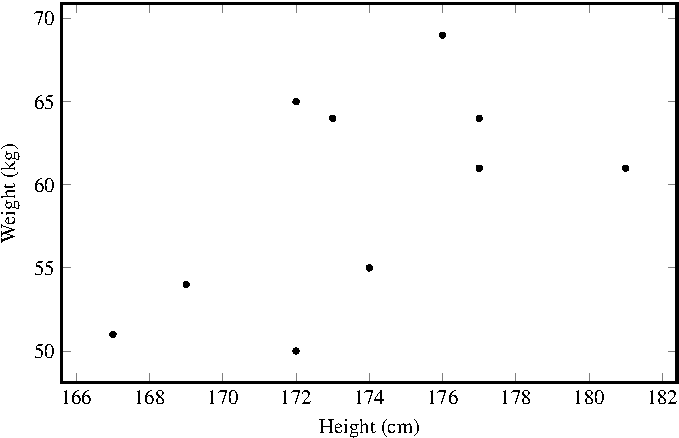
\includegraphics[scale=1]{image/07/height-weight-scatterplot.pdf}
\caption{%%
  A scatter plot of the height versus weight of ten Hong Kong
  teenagers.  The data are from \Table{tab:height_weight}.
}
\label{fig:height_weight_scatterplot}
\end{figure}

\begin{table}[!htbp]
\centering
\begin{tabular}{ccc}                    \toprule
Student & Hours studying & Test score \\\midrule
1       & $4$            & $5$        \\
2       & $3$            & $5$        \\
3       & $6$            & $7$        \\
4       & $2$            & $4$        \\
5       & $1$            & $2$        \\
6       & $5$            & $7$        \\
7       & $8$            & $9$        \\
8       & $9$            & $10$       \\
9       & $4$            & $6$        \\
10      & $10$           & $10$       \\
11      & $7$            & $9$        \\\bottomrule
\end{tabular}

\caption{%%
  The number of hours that eleven students spent on studying for a
  test versus their test scores.  The test is marked out of ten.
}
\label{tab:test_score}
\end{table}

\begin{exercise}
\Table{tab:test_score} shows how many hours that students spent on
studying for a test and their test scores.  Graph the data in the
table as a scatter plot.  What can you conclude from the scatter plot?
\end{exercise}
%%
\ifbool{showSolution}{
\begin{solution}
\Figure{fig:test_score} shows a scatter plot of the data from
\Table{tab:test_score}.  The scatter plot shows that the more time a
student spent on studying for a test, the higher is the student's test
score.

\begin{figure}[!htbp]
\centering
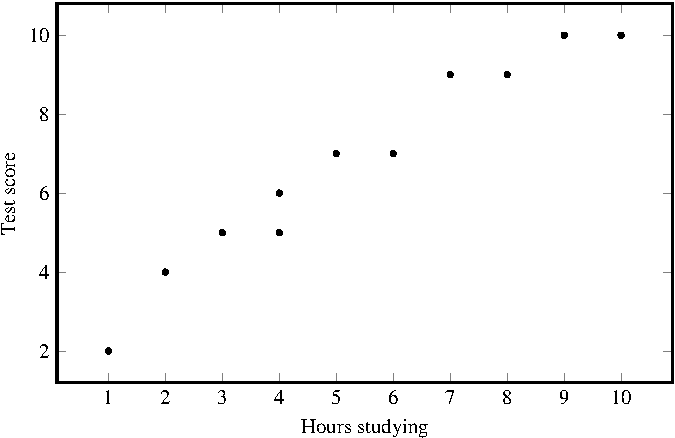
\includegraphics[scale=1]{image/07/test-score-scatterplot.pdf}
\caption{%%
  The number of hours that students spent studying for a test versus
  their test scores.  The data are from \Table{tab:test_score}.
}
\label{fig:test_score}
\end{figure}
\end{solution}
}{}

\begin{table}[!htbp]
\centering
\begin{tabular}{cc} \toprule
Age   & Eggs      \\\midrule
$4$   & $5$       \\
$5$   & $6$       \\
$6$   & $4$       \\
$7$   & $5$       \\
$8$   & $5$       \\
$9$   & $4$       \\
$10$  & $4$       \\
$11$  & $4$       \\
$12$  & $3$       \\
$13$  & $4$       \\
$14$  & $3$       \\
$15$  & $2$       \\
$16$  & $3$       \\
$17$  & $2$       \\\bottomrule
\end{tabular}

\caption{%%
  The age of a hen versus the number of eggs that she laid per week.
  Age is measured in months.
}
\label{tab:age_egg}
\end{table}

\begin{exercise}
\Table{tab:age_egg} shows the age of a hen and the number of eggs that
she laid per week.  Graph the data in the table as a scatter plot.
What can you conclude from the scatter plot?
\end{exercise}
%%
\ifbool{showSolution}{
\begin{solution}
\Figure{fig:age_egg} shows a scatter plot of the data in
\Table{tab:age_egg}.  Without any additional information, apart from
what is presented in the table, the graph shows that as the hen gets
older she lays fewer eggs per week.

\begin{figure}[!htbp]
\centering
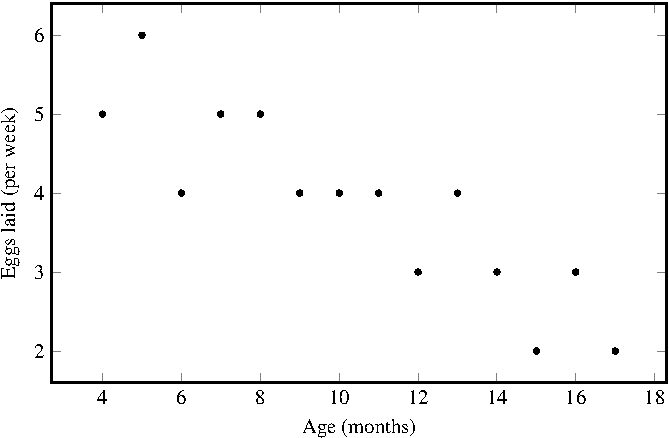
\includegraphics[scale=1]{image/07/age-eggs-scatterplot.pdf}
\caption{%%
  The number of eggs that a hen laid per week versus her age in
  months.  The data are from \Table{tab:age_egg}.
}
\label{fig:age_egg}
\end{figure}
\end{solution}
}{}

\end{document}
